\documentclass[11pt,mathserif]{beamer}
\usepackage{etex}
\usepackage{amsmath}
\usepackage{mathtools}
\usepackage{tikz} 
\usepackage{movie15}
\usepackage{algorithm} % must read after hyperref
\usepackage{algorithmic}
\usepackage{subfigure,MnSymbol,pdfpages}
\usepackage{graphicx,color,colortbl}
\usepackage{bm,amsfonts,graphics}

\newcommand{\vx} {\mathbf{x}}
\newcommand{\vX} {\mathbf{X}}
\newcommand{\vXbar} {\bar{\mathbf{X}}}
\newcommand{\vxbar} {\bar{\mathbf{x}}}

\newcommand{\vf} {\mathbf{f}}
\newcommand{\vy} {\mathbf{y}}
\newcommand{\N} {\mathcal{N}}

\setbeamercolor{block title}{bg=blue!55,fg=black}%bg=background, fg= foreground
\setbeamercolor{block body}{bg=blue!20,fg=black}%bg=background, fg= foreground

\usepackage{amsmath}
\usepackage{mathtools}
\usepackage{tikz}
%\usepackage{movie15}
\usepackage{algorithm} % must read after hyperref
\usepackage{algorithmic}
\usepackage{subfigure,MnSymbol}
\usepackage{graphicx,color,colortbl}
%\usepackage[footnotesize,bf]{caption}
\usepackage{bm,amsfonts,graphics}
\usepackage{tikz,tkz-graph,tkz-arith,tkz-berge}
\usetikzlibrary{arrows,shapes,positioning}

\graphicspath{{./}{figures/}}
\usepackage{multicol}

\newtheorem{thm}{Theorem}
\newtheorem{lem}{Lemma}
\newtheorem{prop}{Proposition}
\newtheorem{rem}{Remark}

\newcommand{\jcols}[4]{
\begin{columns}[T]\begin{column}[T]{#3\textwidth} #1 \end{column}
\begin{column}[T]{#4\textwidth} #2 \end{column}
\end{columns}}

\newcommand{\jcolsb}[4]
{\begin{columns}[b]
\begin{column}{#3\textwidth} #1 \vspace{0pt}
\end{column}
\begin{column}{#4\textwidth} #2 \vspace{0pt}
\end{column}
\end{columns}}

\newcommand{\jcolsc}[4]
{\begin{columns}[c]
\begin{column}{#3\textwidth} #1 \vspace{0pt}
\end{column}
\begin{column}{#4\textwidth} #2 \vspace{0pt}
\end{column}
\end{columns}}
\mode<presentation>
{
	\usetheme{ACL}
        \setbeamercovered{transparent=0}
}

\makeatletter
\newdimen\labelwidthi
\newdimen\labelwidthii
\newdimen\labelwidthiii
\newdimen\labelwidthiv
\def\normal@labelsep{0.2em}
\labelsep\normal@labelsep
\settowidth{\labelwidthi}{iii}
\settowidth{\labelwidthii}{ii}
\settowidth{\labelwidthiii}{iii}
%\settowidth{\labelwidthiv}{i}
\setlength\leftmargini{0pt}
\setlength\leftmarginii{1.5ex}
\setlength\leftmarginiii{1.5ex}

\leftmargini\labelwidthi    \advance\leftmargini\labelsep
\leftmarginii\labelwidthii  \advance\leftmarginii\labelsep
\leftmarginii\labelwidthiii \advance\leftmarginiii\labelsep

%\leftmarginii\labelwidthiv  \advance\leftmarginiv\labelsep
%\def\setleftmargin#1#2{\settowidth{\@tempdima}{#2}\labelsep\normal@labelsep
%  \csname labelwidth#1\endcsname\@tempdima
%  \@tempdimb\@tempdima \advance\@tempdimb\labelsep
%  \csname leftmargin#1\endcsname\@tempdimb}
%\def\@listI{\leftmargin\leftmargini
%  \labelwidth\labelwidthi \labelsep\normal@labelsep
%  \topsep \z@ \partopsep\z@ \parsep\z@ \itemsep\z@
%  \listparindent 1em}
%\def\@listii{\leftmargin\leftmarginii
%  \labelwidth\labelwidthii \labelsep\normal@labelsep
%  \topsep\z@ \partopsep\z@ \parsep\z@ \itemsep\z@
%  \listparindent 1em}
%\def\@listiii{\leftmargin\leftmarginiii
%  \labelwidth\labelwidthiii \labelsep\normal@labelsep
%  \topsep\z@ \partopsep\z@ \parsep\z@ \itemsep\z@
%  \listparindent 1em}
%\def\@listiv{\leftmargin\leftmarginiv
%  \labelwidth\labelwidthiv \labelsep\normal@labelsep
%  \topsep\z@ \partopsep\z@ \parsep\z@ \itemsep\z@
%  \listparindent 1em}
%\let\@listi\@listI
%\@listi
\makeatother

\logo{

\includegraphics[height = 0.6cm,trim=0 50 0 0,clip]{AO-logo-high_color-top-MIT}

\includegraphics[height = 0.5cm,trim=0 0 0 0,clip]{ACL_logo}
}

\setbeamerfont{frametitle}{size=\large,series=\bfseries}
%\setbeamertemplate{frametitle}[default][center]
\setbeamerfont{title}{size=\large,series=\bfseries}
\setbeamerfont{framesubtitle}{series=\mdseries,size=\large}
\graphicspath{{./}{figures/}}
\usepackage[square, numbers, comma]{natbib}	% use Natbib for author-name
									% citations. In a presentation,
									% this is more legible than pure
									% numbers, like [21]. Google
									% "natbib" for more information.
									% Instead of "\cite{abc}", use
									% "\citep{abc}" or "\citet{abc}"
\bibliographystyle{plainnat}		% Natbib specific
%\bibpunct{(}{)}{,}{a}{}{,}			% Natbib specific

\definecolor{Maroon}{RGB}{112,0,0}
\definecolor{Crimson}{RGB}{200,0,0}
\definecolor{purple}{RGB}{112,0,112}

\newcommand{\bee}{\begin{enumerate}}
\newcommand{\eee}{\end{enumerate}}
\newcommand{\bi}{\begin{itemize}}
\newcommand{\bii}{\begin{itemize}\small}
\newcommand{\beee}{\begin{enumerate}\scriptsize}
\newcommand{\biii}{\begin{itemize}\footnotesize}
\newcommand{\ei}{\end{itemize}}
\newcommand{\jtem}{\vfill\item}
\newcommand{\bea}{\begin{eqnarray}}
\newcommand{\eea}{\end{eqnarray}}
\newcommand{\argmax}{\operatornamewithlimits{argmax}}
\newcommand{\njra}{\color{red} $\Rightarrow$~\color{black}}
\newcommand{\nred}[1]{{\tiny \color{red} XX #1 XX\color{black}}}
%\newcommand{\jframe}[1]{\begin{frame}\nred{#1}\end{frame}}
\newcommand{\jframe}[2]{\begin{frame}\frametitle{#1} #2 \end{frame}}
\newcommand{\jframeb}[2]{\begin{frame}[t]{#1} \begin{itemize} #2 \end{itemize} \end{frame}}
\newcommand{\jframet}[2]{\begin{frame}[t]\frametitle{#1} #2 \end{frame}}
\newcommand{\ji}[2]{\begin{itemize}\setlength{\itemsep}{#1mm}{#2}\end{itemize}}
\newcommand{\jen}[2]{\begin{enumerate}\setlength{\itemsep}{#1mm}{#2}\end{enumerate}}
\newcommand{\bc}{\begin{center}}
\newcommand{\ec}{\end{center}}
\newcommand{\todo}[1]{{\color{magenta} XX- #1 -XX}}
\newcommand{\XX}[1]{{\color{red} XX- #1 -XX}}
\newcommand{\alertr}[1]{\textbf{\color{red} #1}}

\setbeamercovered{transparent=10}
\setbeamercolor{title}{bg = black!10}
\setbeamercolor{frametitle}{bg = black!0}
\setbeamercolor{thm}{bg = black!0}
%\setbeamercolor{alerted text}{fg=blue}
%\setbeamerfont{alerted text}{series = \bfseries}

%{use = palette secondary, bg = palette secondary.bg}

\setbeamercolor{normal text}{fg=black}  
\setbeamertemplate{enumerate items}[ball]
\setbeamertemplate{enumerate subitem}{(\alph{enumii})}
\setbeamertemplate{enumerate subsubitems}[triangle]
\setbeamertemplate{itemize item}{$\filledmedtriangleright$}
\setbeamertemplate{itemize subitem}[circle]
\setbeamertemplate{itemize subitem}{\tiny $\stackrel{\color{red}\filledmedsquare\color{black}}{\hbox{\vrule width 0ex height .25ex}}$}

\setbeamertemplate{navigation symbols}{}
\setbeamersize{text margin left=5mm, text margin right=8mm}

\tikzstyle{input} = [coordinate] %
\tikzstyle{block} = [draw, fill=red!20, rectangle, minimum height=3em, minimum width=6em] %
\tikzstyle{block2} = [draw, fill=blue!20, diamond, minimum height=3em, minimum width=6em] %


\title[Current Work]{Gaussian Processes in Autonomy}
\subtitle{Adaptive Control and Adaptive Sensing}

\author[R. Grande]{Robert Grande}

\institute[ACL, MIT]
	{Aerospace Controls Laboratory\\
	Department of Aeronautics \& Astronautics\\
	Massachusetts Institute of Technology} 

\date[\today]{\today}

\iffalse
\AtBeginSection[]
{
	\begin{frame}<beamer>{Outline}
		\tableofcontents[currentsection, hideallsubsections]
	\end{frame}
}
\setcounter{framenumber}{0}
\fi

%LATEX Comments 
%\usepackage[usenames]{color}
%\usepackage[svgnames]{xcolor}
\definecolor{DarkGreen}{rgb}{0,0.5,0}
\definecolor{DarkRed}{rgb}{0.75,0,0}

\renewcommand{\XX}[1]{{\color{red} \bf XX #1 XX\ }}
%\newcommand{\XX}[1]{{\bf XX #1 XX}}
\newcommand{\jsec}[1]{\marginpar{\fcolorbox{yellow}{yellow}{\parbox{0.7in}{\raggedright \color{blue} \tiny #1 }}}}
\newcommand{\hsec}[1]{\marginpar{\fcolorbox{yellow}{yellow}{\parbox{0.7in}{\raggedright \color{green} \tiny #1 }}}}
\newcommand{\jhmargin}[2]{{\color{orange}#1}\marginpar{\color{orange}\tiny\raggedright \bf [JH] #2}}

\begin{document}

\begin{frame}
	\titlepage
\end{frame}

\iftrue
\section*{Outline}
\begin{frame}{Outline}
%\begin{frame}[allowframebreaks]{Outline}

% Use this form for multi-column outline
%\begin{multicols}{2}
%	\tableofcontents[pausesections]
%	%\tableofcontents
%\end{multicols}
% Use this form for multi-column outline

	\tableofcontents %[pausesections]
	%\tableofcontents
\end{frame}
\fi

\section[Gaussian Processes]{Gaussian Processes}
\begin{frame}[t]{Gaussian Processes}
\begin{columns}[T]
	\begin{column}{.5\textwidth}
	\begin{itemize}	\itemsep 0.1in
		\item Framework exists for nonlinear regression known as Gaussian Processes (GPs)

		\item Nonparametric approach which models function as correlation between points
\begin{itemize}
\item Underlying structure can be expressed more freely from data

\end{itemize}
		\item  $p(\vf \mid \vX) = \N (\vf \mid 0, K)$, where
                  $K_{ij} = k(\vx_i, \vx_j)$ is the kernel function
\item Large computational burden as data size increases. Requires offline setting or sparsification.


	\end{itemize}
	\end{column}
	
	\begin{column}{.5\textwidth}
\begin{figure}
	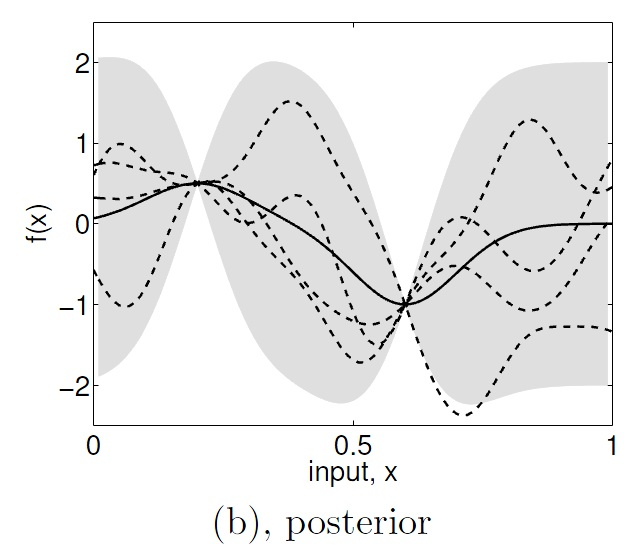
\includegraphics[width=\columnwidth]{figures/GPpost}
\caption{Posterior estimate given GP assumption}
\end{figure}
	\end{column}		
\end{columns}

\end{frame}

\section[Adaptive Sensing]{Adaptive Sensing}
\begin{frame}[t]{Adaptive Sensing}
\bi
\item Problem statement:
\begin{itemize}
\item Given an unknown environment, find efficient way of choosing informative sensing locations using multiple agents such as UAVs
\begin{itemize}
                  \item Ex: Plume tracking, modeling flows in lakes, modeling the formation of a thermal in the atmostphere
		\end{itemize}
\end{itemize}

\item Technical Challenges:
\begin{itemize}
\item Choosing the most informative locations requires checking a combinatorial number of grid points, which is intractable
\item Location selection will depend on the modeling parameters, which are unknown
\item Dynamics of the environment may be changing with time
\end{itemize}
\item Past Approaches
\bi
\item Use a greedy process to sequentially select most informative points using a GP model.
\bi
\item Gives near optimal results, but can be only used for a small subset of problems, known as submodular.
%\item Cannot consider problems with time varying dynamics or environment dependent fuel costs
\ei
\ei
\ei

\end{frame}



\begin{frame}[t]{Adaptive Sensing}
\begin{columns}[T]
	\begin{column}{.5\textwidth}
	\begin{itemize}	\itemsep 0.1in
	\item Our Approach
\bi
		\item Use a GP model for efficient selection using closed form expressions 
		\item Use gradient based optimization 
\bi
			\item Scales comparatively with greedy methods
			\item Allows more flexibility in problem definition
\ei
                \item Training of nonstationary kernel is difficult but results in better waypoint selection 
	\begin{itemize}
                  \item Developed method of training nonstationary
                    kernels with significantly reduced computation time
		\end{itemize}
\ei

	
	\end{itemize}
	\end{column}
	
	\begin{column}{.5\textwidth}
\begin{figure}
	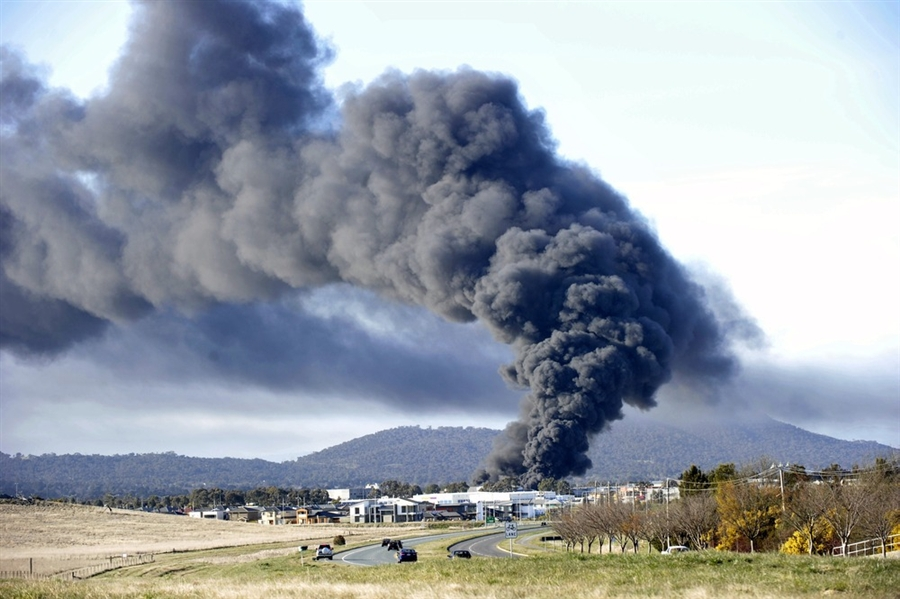
\includegraphics[width=\columnwidth]{figures/plume}
\caption{Toxic Plume from factory fire}
\end{figure}
	\end{column}		
\end{columns}
\end{frame}

\begin{frame}[t]{Results}
\begin{columns}[T]
	\begin{column}{.5\textwidth}

\begin{figure}
	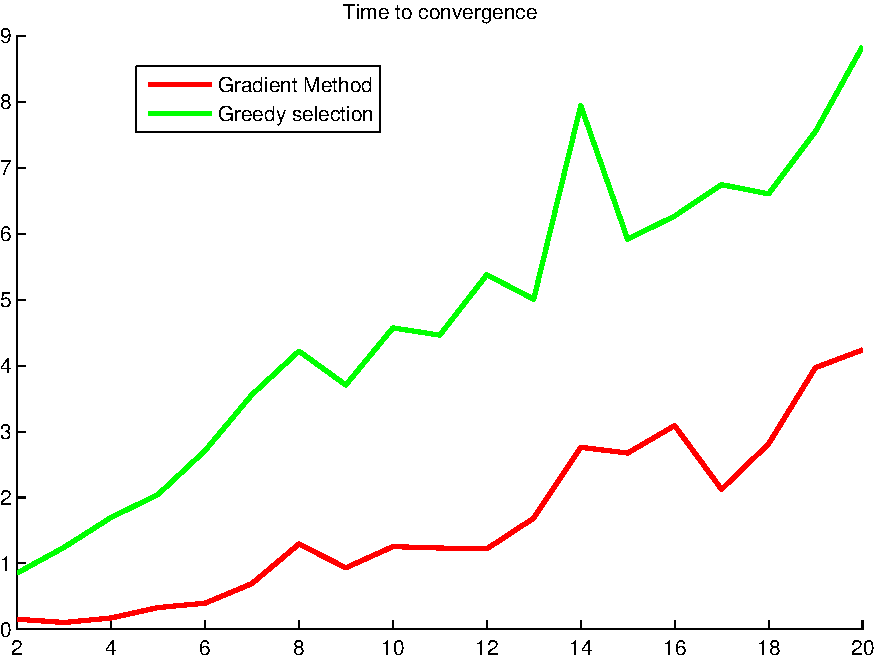
\includegraphics[width=\columnwidth]{figures/Time_sensor.pdf}
\end{figure}
	\end{column}
	
	\begin{column}{.5\textwidth}
\begin{figure}
	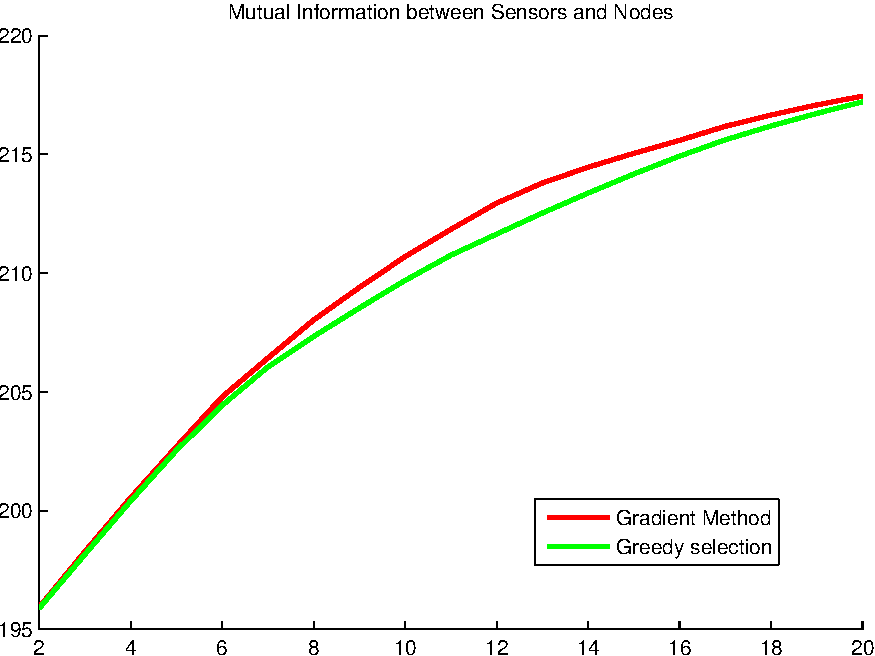
\includegraphics[width=\columnwidth]{figures/MI_sensor.pdf}
\end{figure}
	\end{column}		
\end{columns}
\end{frame}


\begin{frame}[t]{Results}
\begin{figure}
\centering
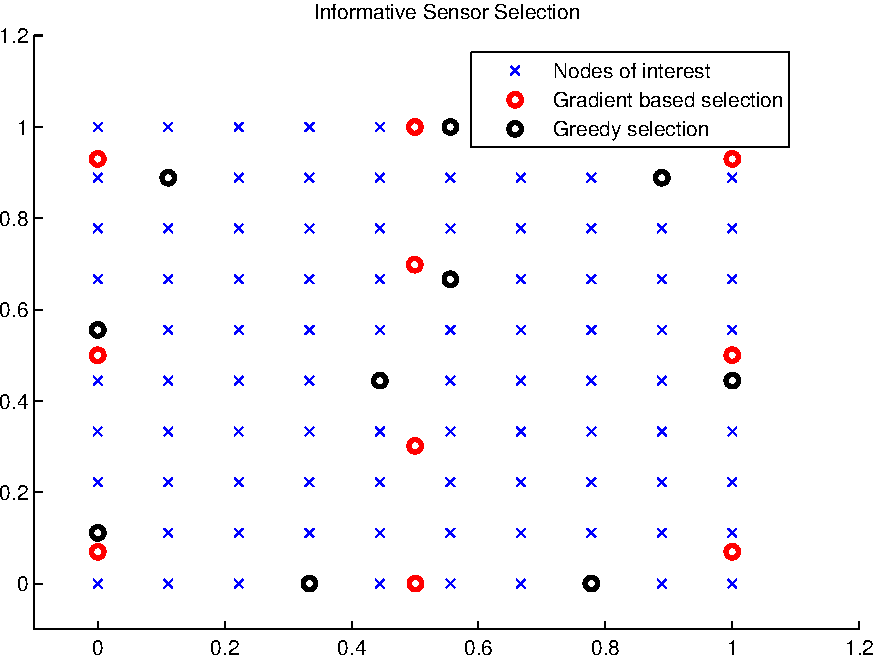
\includegraphics[width=0.7\columnwidth]{figures/SensorLoc.pdf} \caption{Comparison of waypoint selection}
\end{figure}
\end{frame}


\begin{frame}
\huge{Research Topic 2: Adaptive Control}
\end{frame}
\section[GP-MRAC]{Model Reference Adaptive Control}
\begin{frame}[t]{Model Reference Adaptive Control}
\begin{itemize}
\item Goal: control a system with dynamics that are difficult to model or predict
\item Typically, two approaches: direct vs. indirect
  \begin{itemize}
  \item Direct adaptive control attempts to drive tracking error to zero
    by adjusting control gains directly.
  \item Indirect adaptive control models the plant uncertainty and
    adjusts control according to model.
  \end{itemize}
\item In MRAC, popular methods for modeling the uncertainty include
  the Radial Basis Function -Neural Network (RBFN)
  \begin{itemize}
  \item Requires a priori knowledge of the operating domain to
    guarantee coverage
  \item Requires tuning of parameters and center locations offline
  \end{itemize}
\end{itemize}
\end{frame}

\begin{frame}[t]{GP-MRAC Results}
\begin{columns}[T]
	\begin{column}{.5\textwidth}
	\begin{itemize}	\itemsep 0.1in
        \item Recently members of the ACL developed new MRAC framework using GPs for regression.
          \begin{itemize}
          \item Does not require a priori knowledge of the operating
            domain for domain coverage
          \end{itemize}
          \item Requires modifications to original GP framework for
            online feasibility
            \begin{itemize}
\item Sparsification and online center allocation for fast prediction
\end{itemize}
      
	\end{itemize}
	\end{column}
	
	\begin{column}{.5\textwidth}
\begin{figure}
	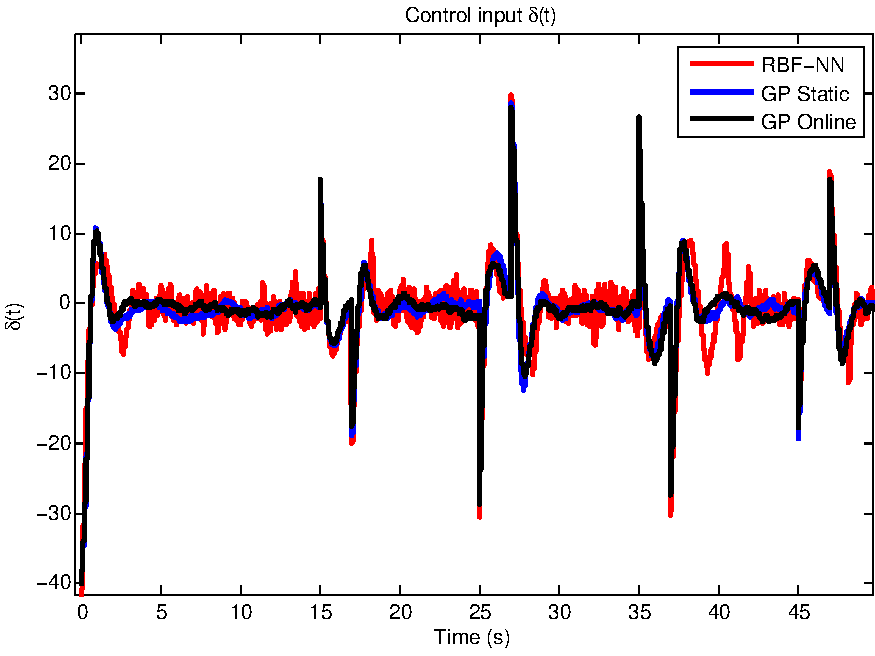
\includegraphics[width=\columnwidth]{figures/ControlInstance.pdf}
\caption{GP-MRAC models the uncertainty better, leading to smoother
  control for a case of tracking roll commands subject to wing rock.}
\end{figure}
	\end{column}		
\end{columns}

\end{frame}



\begin{frame}[t]{CDC 2013 Results}
	\begin{itemize}	\itemsep 0.1in
         \item Submitted paper to the IEEE Conference on Decision
              and Control 2013
          \begin{itemize}
          \item Main contribution: Hyperparameter optimization in an
            online setting
            \item Improves robustness of controller to initialization parameters
          \end{itemize}
	\end{itemize}
\begin{figure}	
\begin{columns}[T]
\begin{column}{.45\textwidth}
\begin{figure}
	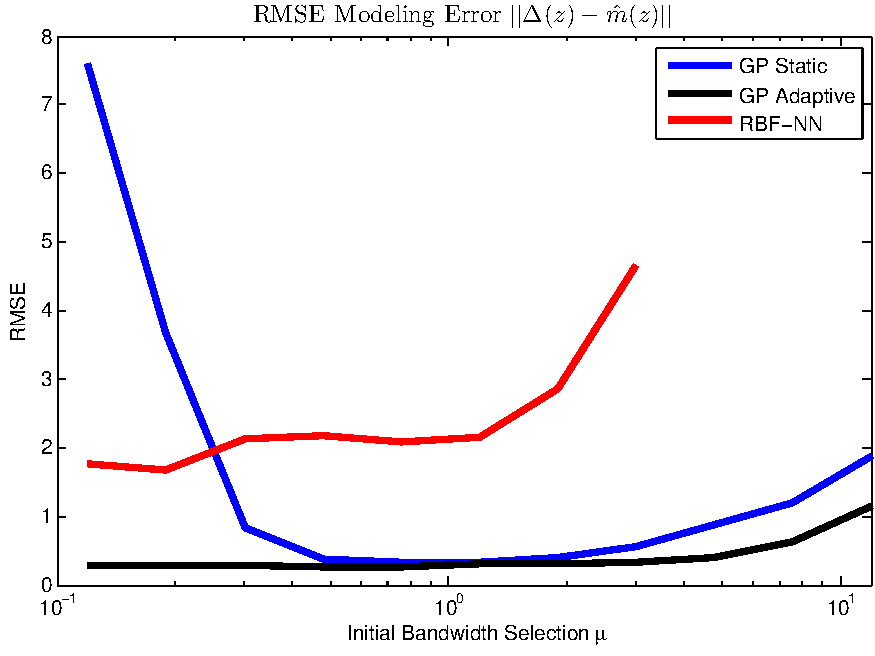
\includegraphics[width=\columnwidth]{figures/RMSE_Model.pdf}
\end{figure}
\end{column}
\begin{column}{.45\textwidth}
\begin{figure}
  	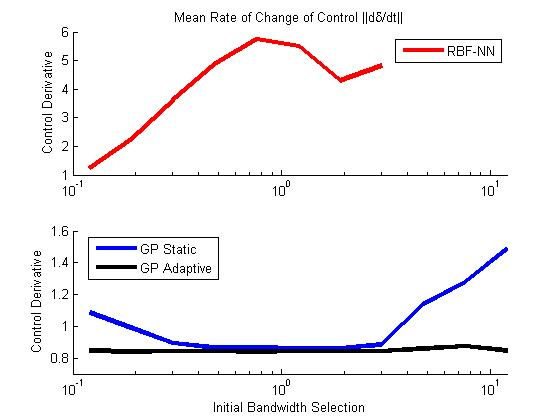
\includegraphics[width=\columnwidth]{figures/ControlD3.jpg}
\end{figure}
\end{column}
\end{columns}
\caption{Hyperparameter optimization results in much more robust
  control performance for tracking commands subject to wing rock dynamics}
\end{figure}


\end{frame}


\section[Future Work]{Future Work}
\begin{frame}[t]{Future Work}
\begin{itemize}
\item Gaussian Processes and Adaptive Sensing
  \begin{itemize}
\item Explore performance compared to greedy methods on bench mark examples
    \item Need means for fast training of nonstationary kernels in
      online setting
      \item Need way of selecting informative sensing locations with
        limited a priori information about the structure of the environment
  \end{itemize}
\item Adaptive Control
  \begin{itemize}
  \item Iterative learning: Improve feed forward performance by updating
    reference model over time or iterations
\item Explorative learning: to learn dynamics efficiently in ``safe" conditions using similar criteria from adaptive sensing
    \item Test GP-MRAC on more difficult dynamics such as the
      Hydrodynamic Cart-Pole, aircraft with non-conventional dynamics, etc.
  \end{itemize}
\end{itemize}


\end{frame}







% Save final frame number, so that backup slides are not counted
\newcounter{finalframe}
\setcounter{finalframe}{\value{framenumber}}

\subsection*{References}
\begin{frame}[allowframebreaks]{References}
	\tiny
	\def\newblock{}
\bibliographystyle{abbrv}
\bibliography{bibifiles/controls,BIB_all/bibtex_database_Chowdhary,bibifiles/bibtex_database_chowdhary_machine_learning,BIB_all/ACL_all,BIB_all/ACL_publications,BIB_all/bibtex_Grande}
\end{frame}

\setcounter{framenumber}{\value{finalframe}}
% Set up so that backup slides are not counted in total slides

\end{document}
